%\subsection{Validation of the methodology}

% \subsection{Testing is simulated scenario}\label{sec:synth}
In order to validate our algorithms we devised a simulated touching environment,
where we performed a number of tests on 9 everyday objects, like bowls, pots, spoons and mugs.
In order to have a ground truth for our tests we used complete point clouds and polygonal meshes of
such objects, those are visible in Figure~\ref{fig:meshes}.

\begin{figure}[htb]
    \centering
    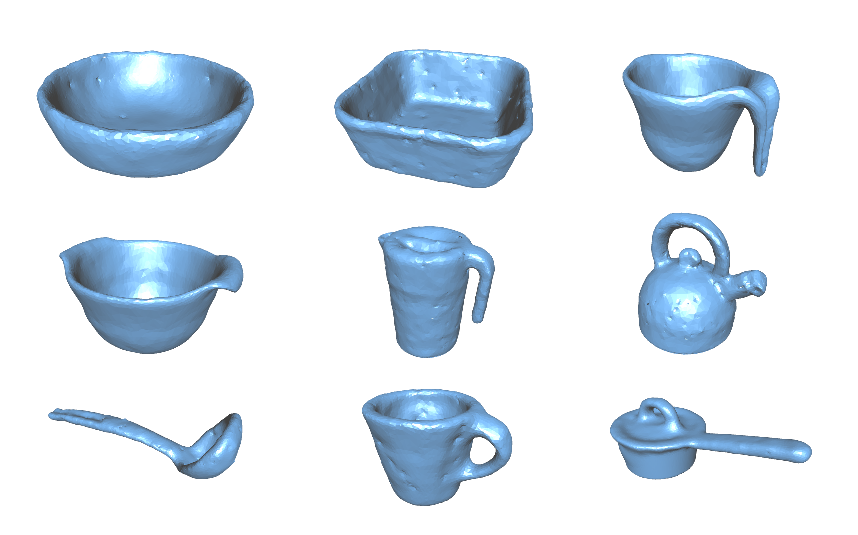
\includegraphics[width=0.95\columnwidth]{meshes.eps}
    \caption{Object meshes used as ground truth for our tests. From top to bottom and from left
    to right: bowlA, bowlB, containerA, containerB, jug, kettle, spoon, mug and pot.}
    \label{fig:meshes}
\end{figure}

These data represents full recontructed shapes and were obtained by means of a common
RGBD sensor and a turn table. The meshes created this way are used as ground thruth 
comparison for shapes reconstructed by our algorithm and at the same time,
are used to extract  partial view point clouds to set as initial training
data ($\mathcal{S}^0$), for our Gaussian Process regression, see Sec.~\ref{sec:gpis}.
It is worth nothing, that the meshes obtained this way are affected by sensor measurements noise 
and they don't perfectly represents the real object shapes. However this is no concern to us, because also the
training sets used in our validations are obtained from the same meshes, thus estimations and ground truth are
consistent with each other.

Each test we performed encloses a full object shape reconstruction and it's carried over
by iterating our \textsc{GPAtlasRRT} algorithm, Alg.~\ref{alg:strategy}~in~Sec.~\ref{sec:solution},
until the shape is predicted with desired variance $\mathbb{V}_{\max} = 0.1$.
% find a solution path that defines the best next tactile action to perform, until

The best next tactile action to perform at each iteration is simulated in our
environment by using  raycasting techniques towards the ground truth mesh.
Rays are uniquely defined by a chart center, as pivot point, and its normal, as direction.
Thus we can define  ray-mesh intersections as touches, i.e. points on surface, and no intersections
as points outside the surface. These new points are used to update the training set
and the GP model, from which a new \textsc{GPAtlasRRT} iteration can take place. 

In order to broaden our tests, we adopted three different tactile actions for each object, consequently forming 
three test groups, for a total of 27 full shape reconstructions. Each test group is described as follows:
\begin{asparadesc}
    \item[Random Touch], for the first test group we ignored the \textsc{GPAtlasRRT} solution path and 
        we just touched a random point on the GP manifold, with the raycasting technique described above.
        The random touching is repeated until the reconstructed shape is correctly predicted with
        desired variance of $0.1$.
        It is worth nothing that we expected these tests to take a fairly high amount of touches
        in order to recontruct the shape and they were performed as a comparison for our method.
        Test results are visible in Table~\ref{tab:test1}.
    \item[Single Poking], for the second test group we actually begin using the \textsc{GPAtlasRRT} solution by
        poking the last chart identified by the path. I.e. we used the raytracing technique applied to the last
        chart of the solution path, performing a touch were the algorithm tells us to go.
        Convergence criteria are the same as the previous test, thus we repeat tactile actions
        until the shape is fully reconstructed. Results in Table~\ref{tab:test2} shows a significant reduction
        in number of tactile actions required, in order to reach requested shape variance.
    \item[Sliding Touch],  for the  final test  category we  decided to  use the
    \textsc{GPAtlasRRT}  full solution  path. Starting  from the  root chart  we
    begin raytracing towards the ground truth mesh and from the touched point we
    reininterpolate a  path towards the next  chart. The new path  is raycasted
    again, while it is being traversed, yielding another point to generate a new interpolated path, and so
    on until we traverse all the charts in the path and we reach the tip of the atlas branch.
    With this technique we mimic a probe that is trying to slide across the surface,
    while trying to maintain contact with it. As the virtual probe slides we can discover
    a fairly significant amount of points on the surface and thus we can add more points to the trainging set
    with a single touch action. For this very reason we expected this test to be the most performing among the three,
    in terms of steps requirements, but also in terms quality of the reconstructed shape.
    Table~\ref{tab:test3} shows this test results, which met our expectations.
\end{asparadesc}
\begin{table}
    \centering
    \begin{tabularx}{0.95\columnwidth}{lccccccr}
        \toprule
        Object &&& & & Steps && RMSE \\
        \midrule
        bowlA &&& & &67 && 0.0025\\
        bowlB &&& & &38 && 0.0038\\
        containerA &&&&& 124 && 0.0033\\
        containerB &&&&& 68 && 0.0062\\
        jug &&&&& 106 && 0.0027\\
        kettle &&&&& 98 && 0.0031\\
        spoon &&&&& 35 && 0.0058\\
        mug &&&&& 238 && 0.0017\\
        pot &&&&& 33 && 0.0035\\
        \midrule
        \textbf{Mean} &&&&& $\sim$\textbf{90} && \textbf{0.0036}\\
        \bottomrule
    \end{tabularx}
    \caption{Random Touch test results in terms of the required
    number of actions (Steps) and the Root Mean Squared Error (RMSE) between
    the predicted shape and the ground truth mesh.}
    \label{tab:test1}
\end{table}
\begin{table}
    \centering
    \begin{tabularx}{0.95\columnwidth}{lccccccr}
        \toprule
        Object &&& & & Steps && RMSE \\
        \midrule
        bowlA &&& & &27 && 0.0023\\
        bowlB &&& & &18 && 0.0036\\
        containerA &&&&& 20 && 0.0035\\
        containerB &&&&& 19 && 0.0043\\
        jug &&&&& 20 && 0.003\\
        kettle &&&&& 17 && 0.0032\\
        spoon &&&&& 10 && 0.0055\\
        mug &&&&& 28 && 0.0020\\
        pot &&&&& 12 && 0.0032\\
        \midrule
        \textbf{Mean} &&&&& $\sim$\textbf{19} && \textbf{0.0034}\\
        \bottomrule
    \end{tabularx}
    \caption{Single Poking test results in terms of the required
    number of actions (Steps) and the Root Mean Squared Error (RMSE) between
    the predicted shape and the ground truth mesh.}
    \label{tab:test2}
\end{table}
\begin{table}
    \centering
    \begin{tabularx}{0.95\columnwidth}{lccccccr}
        \toprule
        Object & & &&& Steps && RMSE \\
        \midrule
        bowlA &&& & &8 && 0.0015\\
        bowlB & &&& &5 && 0.0028\\
        containerA &&&&& 11 && 0.0028\\
        containerB &&&&& 8 && 0.0026\\
        jug &&&&& 9 && 0.0025\\
        kettle &&&&& 9 && 0.0029\\
        spoon &&&&& 8 && 0.0031\\
        mug &&&&& 12 && 0.0018\\
        pot &&&&& 6 && 0.0028\\
        \midrule
        \textbf{Mean} &&&&& $\sim$\textbf{8} && \textbf{0.0025}\\
        \bottomrule
    \end{tabularx}
    \caption{Sliding Touch test results in terms of the required
    number of actions (Steps) and the Root Mean Squared Error (RMSE) between
    the predicted shape and the ground truth mesh.}
    \label{tab:test3}
\end{table}

The three set of experiments clearly shows the superiority of our method in terms of number of required steps
and in terms of quality of produced mesh. As a final benchmarking, Table~\ref{tab:comp} summarizes the comparison
between the test methods and Fig.~\ref{fig:shapecomp} shows some  of the \textsc{GPAtlasRRT} Sliding Touch reconstructed shapes with
the ground truth meshes next to them.
\begin{table}
    \centering
    \begin{tabularx}{0.95\columnwidth}{lccccr}
        \toprule
        Tests  &&& Mean Steps && Mean RMSE \\
        \midrule
        Random Touch & & &90 && 0.0036\\
        Single Poking && &19 && 0.0034\\
        Sliding Touch &&& 8 && 0.0025\\
        \bottomrule
    \end{tabularx}
    \caption{Overall comparison: GPAtlasRRT with Sliding Touch outperforms in terms
    of efficiency and accuracy.}
    \label{tab:comp}
\end{table}
\begin{figure}[htb]
    \centering
    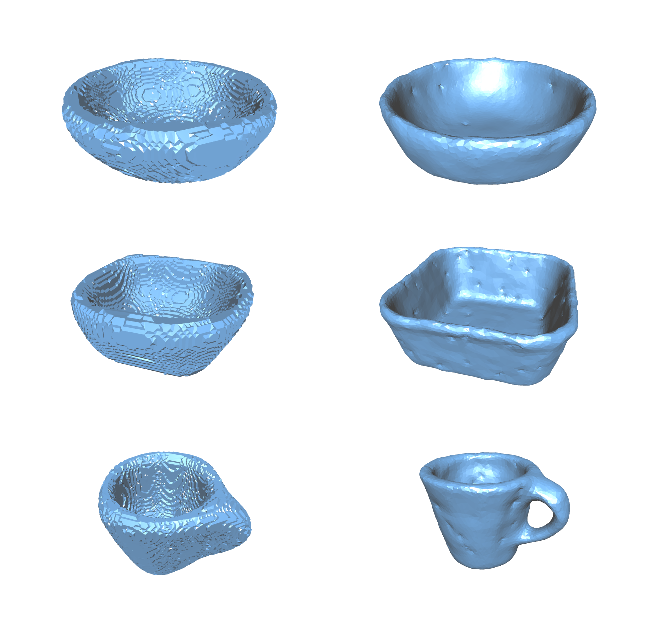
\includegraphics[width=0.95\columnwidth]{comparison.eps}
    \caption{Comparison of reconstructed shapes with the ground truth meshes, obtained with our GPAtlasRRT via the Sliding Touch (left).}
    \label{fig:shapecomp}
\end{figure}

Additionaly, while we performed our validation, we also recorded some videos of shape reconstructions, visible online at \texttt{goo.gl/4GKYTp}.

\vspace{-2em}
\subsection{A real tactile exploration}
\label{sec:real}

The purpose of this test is to illustrate with an example an implementation of Algorithm \ref{alg:solution}, since the real tactile exploration poses more a technical challenge than a scientific contribution when ported into a real scenario. The complete software implementation, as well as this document, is freely available under mixed open-source licensees\footnote{\texttt{github.com/CentroEPiaggio/pacman-DR54}}, heavily-based on the Robot Operating System \citet{ROS}. Note how the GPAtlasRRT from Algorithm \ref{alg:strategy} is part of it as a submodule\footnote{\texttt{github.com/pacman-project/gaussian-object-modelling}}. As with the validation results, the qualitative outcome under the real scenario are better appreciated at \texttt{https://goo.gl/4GKYTp}. The technical details are briefly described next.

In this scenario, we count on our Vito robot, a bimanual robot equipped with 2 KUKA LWR 4+, one Pisa/IIT SoftHand~\citet{Catalano2014Adaptive} as one end-effector, and the intrinsic tactile sensor configuration as introduced by \citet{Rosales2014Active}. We start the experiments by handing an object to its hand. Afterwards, the object is segmented with the help of the recently developed IMU-based glove by \citet{Santaera2015Lowcost} to measure the hand configuration, and remove all the robot geometry from the scene. Other typical filters are applied like pass-through and down-sampling to speed-up the overall pipeline. The acquired cloud at this point contains a partial view of the object and constitutes the initial training data for the Gaussian process, namely $\mathcal{S}^0$. Fig. \ref{fig:real} shows the initial model out of it, then a sequence of touches are performed to finally get to a better model. It is worth noting that, the fact that there is a hand occluding part of the object that is needed to explore impedes to complete the model to a given accuracy, and an additional ending condition by number of failed consecutive attempts is given as it might not be possible to refine areas occluded by the hand.

The setup included three standard personal computers where one was dedicated to the GPAtlasRRT strategy, one acted as the decision-maker and the last as the hardware server. Most of the time is consumed on the computation of the explicit form of the object for collision-avoidance motion planning. Basically, a suggested tactile exploration could be discarded due to accessibility (collision-free and kinematic feasible configurations). In such situation, simply another next-best candidate(s) is requested. Note that, both the GPAtlasRRT strategy and the motion planner are probabilistic, and their combination yielded in some cases behaved like if the algorithm get trapped in a local-minima.

\begin{figure}
\centering
%\mbox{
  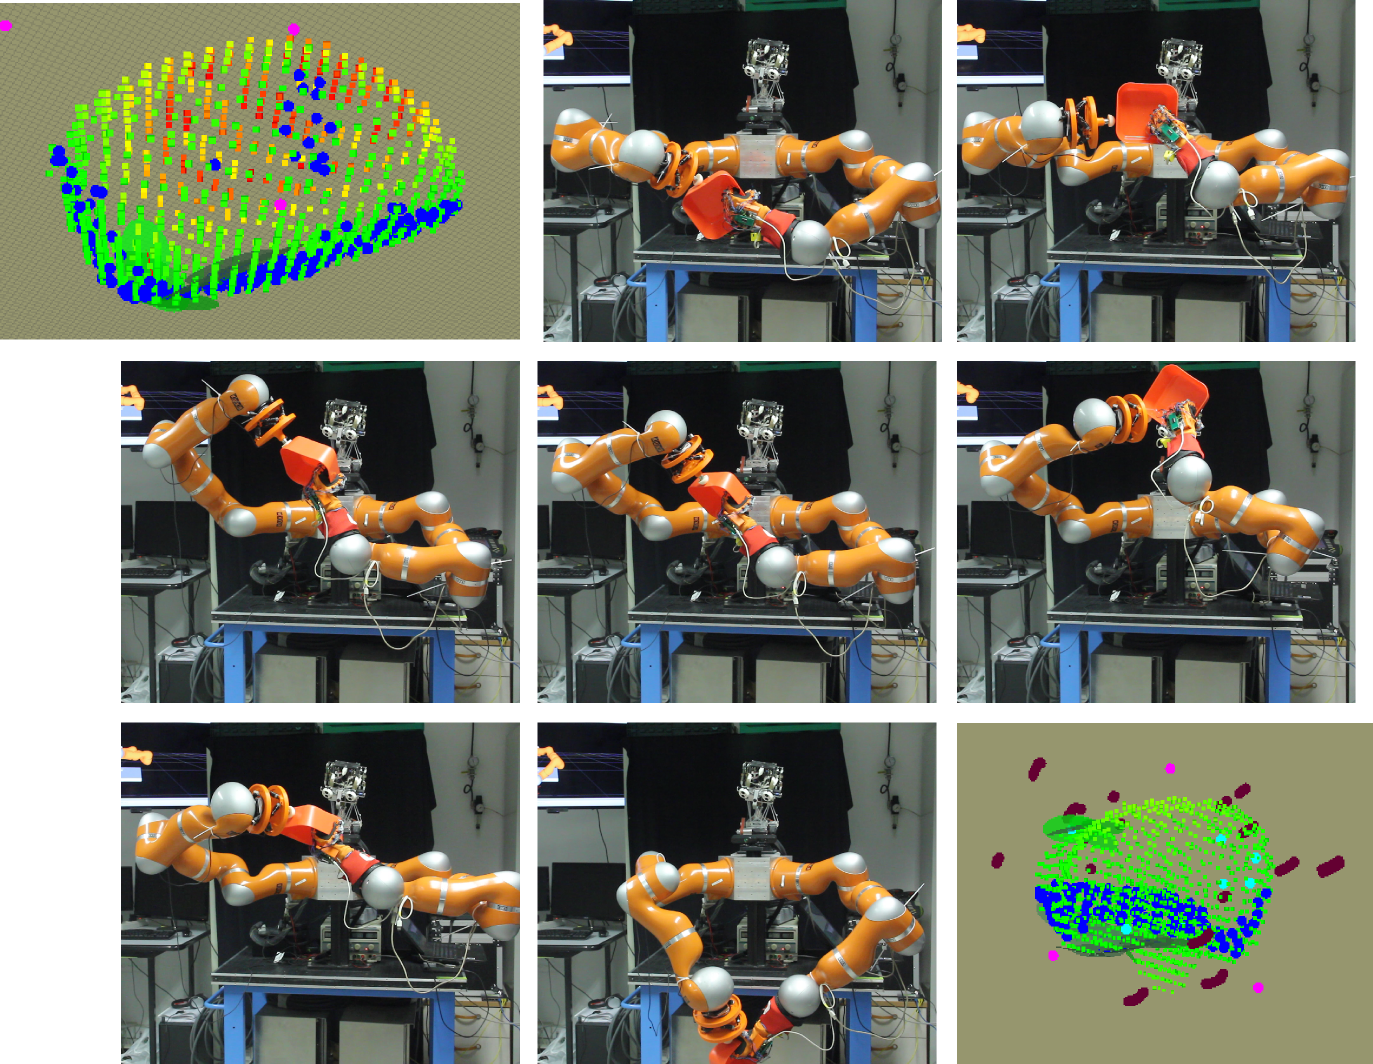
\includegraphics[width=0.9\linewidth]{real_shots.png}
%}
\caption{Our Vito robot performs a tactile exploration using the proposed GPAtlasRRT strategy.}
\label{fig:real}
\end{figure}